\documentclass[../conclusions.tex]{subfiles}

\begin{document}
    
\section{A first estimate of aneurysm rupture risk}

\subsection{Estimating tissue strenght based on a uniaxial tensile test}

The tissue strenght is here defined as the ultimate stress value obtained in a uniaxial tensile test, before damage occurs. Since uniaxial 
tensile tests were performed on circumferentially ($P^{ult}_{\theta\theta}$) as well as axially ($P^{ult}_{zz}$) oriented samples, we can define the strength 
in the circumferential as well as in the axial direction.  

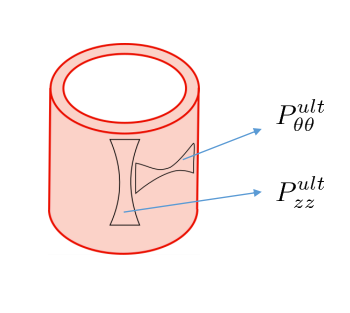
\includegraphics[scale=0.5]{tissue_example.png}



\end{document}